% !TeX spellcheck = en_US
% Dieses Dokument muss mit PDFLatex gesetzt werden
% Vorteil: Grafiken koennen als jpg, png, ... verwendet werden
%          und die Links im Dokument sind auch gleich richtig
%
%Ermöglicht \\ bei der Titelseite (z.B. bei supervisor)
%Siehe https://github.com/latextemplates/uni-stuttgart-cs-cover/issues/4
\RequirePackage{kvoptions-patch}

%Englisch:
\let\ifdeutsch\iffalse
\let\ifenglisch\iftrue

%Deutsch:
%\let\ifdeutsch\iftrue
%\let\ifenglisch\iffalse

%
\ifdeutsch
	\PassOptionsToClass{numbers=noenddot}{scrbook}
\fi

%Warns about outdated packages and missing caption delcarations
%See https://www.ctan.org/pkg/nag
\RequirePackage[l2tabu, orthodox]{nag}

%Neue deutsche Trennmuster
%Siehe http://www.ctan.org/pkg/dehyph-exptl und http://projekte.dante.de/Trennmuster/WebHome
%Nur für pdflatex, nicht für lualatex
\RequirePackage{ifluatex}
\ifluatex
%do not load anything
\else
	\ifdeutsch
		\RequirePackage[ngerman=ngerman-x-latest]{hyphsubst}
	\fi
\fi

\documentclass[
               fontsize=12pt, %Default: 11pt, bei Linux Libertine zu klein zum Lesen
% BEGINN: Optionen für typearea
               paper=a4,
               twoside, % fuer die Betrachtung am Schirm ungeschickt
               BCOR=3mm, % Hack für BCOR (1.92 o.ä.), da bei BCOR2mm die Fuellpunkte beim Inhaltsverzeichnis falsch sind. Hack aber nicht mehr nötig: microtype für Verzeichnisse ausschalten hilft.
               DIV=13,   % je höher der DIV-Wert, desto mehr geht auf eine Seite. Gute werde sind zwischen DIV=12 und DIV=15
               headinclude=true,
               footinclude=false,
% ENDE: Optionen für typearea
%               titlepage,
               bibliography=totoc,
%               idxtotoc,   %Index ins Inhaltsverzeichnis
%                liststotoc, %List of X ins Inhaltsverzeichnis, mit liststotocnumbered werden die Abbildungsverzeichnisse nummeriert
               headsepline,
               cleardoublepage=empty,
               parskip=half,
%               draft    % um zu sehen, wo noch nachgebessert werden muss - wichtig, da Bindungskorrektur mit drin
               final   % ACHTUNG! - in pagestyle.tex noch Seitenstil anpassen
               ]{scrbook}

%%%
% Beschreibung:
% In dieser Datei werden zuerst die benoetigten Pakete eingebunden und
% danach diverse Optionen gesetzt. Achtung Reihenfolge ist entscheidend!
%
%%%


%%%
% Styleguide:
%
% Ein sehr kleiner Styleguide. Packages werden in Blöcken organisiert.
% Ein Block beginnt mit drei % in einer Zeile, dann % <Blocküberschrift>, dann
% eine Liste der möglichen Optionen und deren Einstellungen, Gründe und Kommentare
% eine % Zeile in der sonst nichts steht und dann wieder %%% in einer Zeile.
%
% Zwischen zwei Blöcken sind 2 Leerzeilen!
% Zu jedem Paket werden soviele Optionen wie möglich/nötig angegeben
%
%%%


%%%
% Codierung
% Wir sind im 21 Jahrhundert, utf-8 löst so viele Probleme.
%
% Mit UTF-8 funktionieren folgende Pakete nicht mehr. Bitte beachten!
%   * fancyvrb mit §
%   * easylist -> http://www.ctan.org/tex-archive/macros/latex/contrib/easylist/
\ifluatex
%no package loading required
\else
\usepackage[utf8]{inputenc}
\fi
%
%%%


%%%
% Deckblattstyle
%
\ifdeutsch
\PassOptionsToPackage{language=german}{uni-stuttgart-cs-cover}
\else
\PassOptionsToPackage{language=english}{uni-stuttgart-cs-cover}
\fi

\newcommand{\docauthor}{Jan Ruthardt\\
						Nico Poier\\
						Thomas Breunig}
\newcommand{\doctitle}{Evaluating Open-source Tool Stacks for Application Performance
	Diagnostics}

\usepackage[
title={\doctitle},
author={\docauthor},
type=Fachstudie,
institute=isterss,
number=12345,
course=se,
examiner={Dr.-Ing.\ Andr\'{e} van Hoorn },
supervisor={Thomas F. Düllmann M.Sc.,\\Teerat Pitakrat,\ M.Sc.},
startdate={August 14, 2017}, % English: July 5, 2013;    ISO: 2013-07-05
enddate={February 14, 2018}, % English: January 5, 2014; ISO: 2014-01-05
crk={I.7.2}
]{uni-stuttgart-cs-cover}
%
%%%


%%%
%Parallelbetrieb tex4ht und pdflatex
\makeatletter
\@ifpackageloaded{tex4ht}{\def\iftex4ht{\iftrue}}
                         {\def\iftex4ht{\iffalse}}
\makeatother
%%%


%%%
%Farbdefinitionen
\usepackage[hyperref,dvipsnames]{xcolor}
%


%%%
% Neue deutsche Rechtschreibung und Literatur statt "Literature", Nachfolger von ngerman.sty
\ifdeutsch
% letzte Sprache ist default, Einbindung von "american" ermöglicht \begin{otherlanguage}{amercian}...\end{otherlanguage} oder \foreignlanguage{american}{Text in American}
% see also http://tex.stackexchange.com/a/50638/9075
\usepackage[american,ngerman]{babel}
% Ein "abstract" ist eine "Kurzfassung", keine "Zusammenfassung"
\addto\captionsngerman{%
	\renewcommand\abstractname{Kurzfassung}%
}
\else
%
%
% if you are writing in english
% last language is the default language
\usepackage[ngerman,american]{babel}
\fi
%
%%%

%%%
% Anführungszeichen
% Zitate in \enquote{...} setzen, dann werden automatisch die richtigen Anführungszeichen verwendet.
\usepackage{csquotes}
%%%


%%%
% erweitertes Enumerate
\usepackage{paralist}
%
%%%


%%%
% fancyheadings (nicht nur) fuer koma
\usepackage[automark]{scrpage2}
%
%%%


%%%
%Mathematik
%
\usepackage[fleqn,leqno]{amsmath} % Viele Mathematik-Sachen: Doku: /usr/share/doc/texmf/latex/amsmath/amsldoc.dvi.gz
%fleqn (=Gleichungen linksbündig platzieren) funktioniert nicht direkt. Es muss noch ein Patch gemacht werden:
\addtolength\mathindent{1em}%work-around ams-math problem with align and 9 -> 10
\usepackage{mathtools} %fixes bugs in AMS math
%
%for theorems, replacement for amsthm
\usepackage[amsmath,hyperref]{ntheorem}
\theorempreskipamount 2ex plus1ex minus0.5ex
\theorempostskipamount 2ex plus1ex minus0.5ex
\theoremstyle{break}
\newtheorem{definition}{Definition}[section]
%
%%%


%%%
% Intelligentes Leerzeichen um hinter Abkürzungen die richtigen Abstände zu erhalten, auch leere.
% siehe commands.tex \gq{}
\usepackage{xspace}
%Macht \xspace und \enquote kompatibel
\makeatletter
\xspaceaddexceptions{\grqq \grq \csq@qclose@i \} }
\makeatother
%
%%%


%%%
% Anhang
\usepackage{appendix}
%[toc,page,title,header]
%
%%%


%%%
% Grafikeinbindungen
\usepackage{graphicx}%Parameter "pdftex" unnoetig
\graphicspath{{\getgraphicspath}}
\newcommand{\getgraphicspath}{graphics/}
%
%%%


%%%
% Enables inclusion of SVG graphics - 1:1 approach
% This is NOT the approach of http://www.ctan.org/tex-archive/info/svg-inkscape,
% which allows text in SVG to be typeset using LaTeX
% We just include the SVG as is
\usepackage{epstopdf}
\epstopdfDeclareGraphicsRule{.svg}{pdf}{.pdf}{%
  inkscape -z -D --file=#1 --export-pdf=\OutputFile
}
%
%%%


%%%
% Enables inclusion of SVG graphics - text-rendered-with-LaTeX-approach
% This is the approach of http://www.ctan.org/tex-archive/info/svg-inkscape,
\newcommand{\executeiffilenewer}[3]{%
\IfFileExists{#2}
{
%\message{file #2 exists}
\ifnum\pdfstrcmp{\pdffilemoddate{#1}}%
{\pdffilemoddate{#2}}>0%
{\immediate\write18{#3}}
\else
{%\message{file up to date #2}
}
\fi%
}{
%\message{file #2 doesn't exist}
%\message{argument: #3}
%\immediate\write18{echo "test" > xoutput.txt}
\immediate\write18{#3}
}
}
\newcommand{\includesvg}[1]{%
\executeiffilenewer{#1.svg}{#1.pdf}%
{
inkscape -z -D --file=\getgraphicspath#1.svg %
--export-pdf=\getgraphicspath#1.pdf --export-latex}%
\input{\getgraphicspath#1.pdf_tex}%
}


%%%
\usepackage{siunitx}
%%%

%%%
\usepackage{acro} %nice Acronyms
%\DeclareAcronym{TCT}{short = TCT , long = task completion time}
%%%


%%%
% Tabellenerweiterungen
\usepackage{array} %increases tex's buffer size and enables ``>'' in tablespecs
\usepackage{longtable}
\usepackage{dcolumn} %Aligning numbers by decimal points in table columns
\ifdeutsch
	\newcolumntype{d}[1]{D{.}{,}{#1}}
\else
	\newcolumntype{d}[1]{D{.}{.}{#1}}
\fi

%
%%%

%%%
% Eine Zelle, die sich über mehrere Zeilen erstreckt.
% Siehe Beispieltabelle in Kapitel 2
\usepackage{multirow}
%
%%%

%%%
%Fuer Tabellen mit Variablen Spaltenbreiten
%\usepackage{tabularx}
%\usepackage{tabulary}
%
%%%


%%%
% Links verhalten sich so, wie sie sollen
\usepackage{url}
%
%Use text font as url font, not the monospaced one
%see comments at http://tex.stackexchange.com/q/98463/9075
\urlstyle{same}
%
%Hint by http://tex.stackexchange.com/a/10419/9075
\makeatletter
\g@addto@macro{\UrlBreaks}{\UrlOrds}
\makeatother
%
%%%


%%%
% Index über Begriffe, Abkürzungen
%\usepackage{makeidx} makeidx ist out -> http://xindy.sf.net verwenden
%
%%%

%%%
%lustiger Hack fuer das Abkuerzungsverzeichnis
%nach latex durchlauf folgendes ausfuehren
%makeindex ausarbeitung.nlo -s nomencl.ist -o ausarbeitung.nls
%danach nochmal latex
%\usepackage{nomencl}
%    \let\abk\nomenclature %Deutsche Ueberschrift setzen
%          \renewcommand{\nomname}{List of Abbreviations}
%        %Punkte zw. Abkuerzung und Erklaerung
%          \setlength{\nomlabelwidth}{.2\hsize}
%          \renewcommand{\nomlabel}[1]{#1 \dotfill}
%        %Zeilenabstaende verkleinern
%          \setlength{\nomitemsep}{-\parsep}
%    \makenomenclature
%
%%%

%%%
% Logik für Tex
\usepackage{ifthen} %fuer if-then-else @ commands.tex
%
%%%


%%%
%
\usepackage{listings}
%
%%%


%%%
%Alternative zu Listings ist fancyvrb. Kann auch beides gleichzeitig benutzt werden.
\usepackage{fancyvrb}
%\fvset{fontsize=\small} %Groesse fuer den Fliesstext. Falls deaktiviert: \normalsize
%Funktioniert mit UTF-8 nicht mehr
%\DefineShortVerb{\§} %Somit kann im Text ganz einfach |verbatim| text gesetzt werden.
\RecustomVerbatimEnvironment{Verbatim}{Verbatim}{fontsize=\footnotesize}
\RecustomVerbatimCommand{\VerbatimInput}{VerbatimInput}{fontsize=\footnotesize}
%
%%%


%%%
% Bildunterschriften bei floats genauso formatieren wie bei Listings
% Anpassung wird unten bei den newfloat-Deklarationen vorgenommen
% https://www.ctan.org/pkg/caption2 is superseeded by this package.
\usepackage{caption}
%
%%%


%%%
% Ermoeglicht es, Abbildungen um 90 Grad zu drehen
% Alternatives Paket: rotating Allerdings wird hier nur das Bild gedreht, während bei lscape auch die PDF-Seite gedreht wird.
%Das Paket lscape dreht die Seite auch nicht
\usepackage{pdflscape}
%
%%%


%%%
% Fuer listings
% Wird für fancyvrb und für lstlistings verwendet
\usepackage{float}

%\usepackage{floatrow}
%% zustäzlich für den Paramter [H] = Floats WIRKLICH da wo sie deklariert wurden paltzieren - ganz ohne Kompromisse
% floatrow ist der Nachfolger von float
% Allerdings macht floatrow in manchen Konstellationen Probleme. Deshalb ist das Paket deaktiviert.
%
%%%



%%%
% Fuer Abbildungen innerhalb von Abbildungen
% Ersetzt das Paket subfigure
%
% Due to bug #24 in the caption package we need to update caption3.sty at the moment manualy to use subfig.
% Bug #24: http://sourceforge.net/p/latex-caption/tickets/24/
% corrected caption3.sty: http://sourceforge.net/p/latex-caption/code/HEAD/tree/branches/3.3/tex/caption3.sty
%
\usepackage[caption=false, lofdepth=1, lotdepth]{subfig}
%
%%%




%%%
% Fußnoten
%
%\usepackage{dblfnote}  %Zweispaltige Fußnoten
%
% Keine hochgestellten Ziffern in der Fußnote (KOMA-Script-spezifisch):
%\deffootnote[1.5em]{0pt}{1em}{\makebox[1.5em][l]{\bfseries\thefootnotemark}}
%
% Abstand zwischen Fußnoten vergrößern:
%\setlength{\footnotesep}{.85\baselineskip}
%
%
\renewcommand{\footnoterule}{}             % Keine Trennlinie zur Fußnote
\addtolength{\skip\footins}{\baselineskip} % Abstand Text <-> Fußnote
% Fußnoten immer ganz unten auf einer \raggedbottom-Seite
\usepackage{fnpos}
%
%%%


%%%
%
\raggedbottom     % Variable Seitenhöhen zulassen
%
%%%


%%%
% Falls die Seitenzahl bei einer Referenz auf eine Abbildung nur dann angegeben werden soll,
% falls sich die Abbildung nicht auf der selben Seite befindet...
\iftex4ht
%tex4ht does not work well with vref, therefore we emulate vref behavior
\newcommand{\vref}[1]{\ref{#1}}
\else
\ifdeutsch
\usepackage[ngerman]{varioref}
\else
\usepackage{varioref}
\fi
\fi
%%%

%%%
% Noch schoenere Tabellen als mit booktabs mit http://www.zvisionwelt.de/downloads.html
\usepackage{booktabs}
%
%\usepackage[section]{placeins}
%
%%%


%%%
%Fuer Graphiken. Allerdings funktioniert es nicht zusammen mit pdflatex
%\usepackage{gastex} % \tolarance kann dann nicht mehr umdefiniert werden
%
%%%


%%%
%
%\usepackage{multicol}
%\usepackage{setspace} % kollidiert mit diplomarbeit.sty
%
%http://www.tex.ac.uk/cgi-bin/texfaq2html?label=floats
%\usepackage{flafter} %floats IMMER nach ihrer Deklaration platzieren
%
%%%


%%%
%schoene TODOs
\usepackage{todonotes}
\let\xtodo\todo
\renewcommand{\todo}[1]{\xtodo[inline,color=black!5]{#1}}
\newcommand{\utodo}[1]{\xtodo[inline,color=green!5]{#1}}
\newcommand{\itodo}[1]{\xtodo[inline]{#1}}
%
%%%


%%%
%biblatex statt bibtex
\usepackage[
  backend       = biber, 	%biber dose not work with 64x versions alternative: bibtex8
														%minalphanames only works with biber backend														
  sortcites     = true,
  bibstyle      = alphabetic,
  citestyle     = alphabetic,
  firstinits    = true,
  useprefix     = false, %"von, van, etc." will be printed, too. See below.
  minnames      = 1,
  minalphanames = 3,
  maxalphanames = 4,
  maxbibnames   = 99,
  maxcitenames  = 3,
	natbib        = true,
	eprint        = true,
	url           = true,
  doi           = true,
  isbn          = true,
  backref       = true]{biblatex}
\bibliography{bibliography}
%\addbibresource[datatype=bibtex]{bibliography.bib}

%Do not put "vd" in the label, but put it at "\citeauthor"
%Source: http://tex.stackexchange.com/a/30277/9075
\makeatletter
\AtBeginDocument{\toggletrue{blx@useprefix}}
\AtBeginBibliography{\togglefalse{blx@useprefix}}

%Thin spaces between initials
%http://tex.stackexchange.com/a/11083/9075
\renewrobustcmd*{\bibinitdelim}{\,}

%Keep first and last name together in the bibliography
%http://tex.stackexchange.com/a/196192/9075
\renewcommand*\bibnamedelimc{\addnbspace}
\renewcommand*\bibnamedelimd{\addnbspace}

%Replace last "and" by comma in bibliography
%See http://tex.stackexchange.com/a/41532/9075
\AtBeginBibliography{%
  \renewcommand*{\finalnamedelim}{\addcomma\space}%
}

\DefineBibliographyStrings{ngerman}{
  backrefpage  = {zitiert auf S\adddot},
  backrefpages = {zitiert auf S\adddot},
  andothers    = {et\ \addabbrvspace al\adddot},
  %Tipp von http://www.mrunix.de/forums/showthread.php?64665-biblatex-Kann-%DCberschrift-vom-Inhaltsverzeichnis-nicht-%E4ndern&p=293656&viewfull=1#post293656
  bibliography = {Literaturverzeichnis}
}

%enable hyperlinked author names when using \citeauthor
%source: http://tex.stackexchange.com/a/75916/9075
\DeclareCiteCommand{\citeauthor}
  {\boolfalse{citetracker}%
   \boolfalse{pagetracker}%
   \usebibmacro{prenote}}
  {\ifciteindex
     {\indexnames{labelname}}
     {}%
   \printtext[bibhyperref]{\printnames{labelname}}}
  {\multicitedelim}
  {\usebibmacro{postnote}}

%natbib compatibility
%\newcommand{\citep}[1]{\cite{#1}}
%\newcommand{\citet}[1]{\citeauthor{#1} \cite{#1}}
%Beginning of sentence - analogous to cleveref - important for names such as "zur Muehlen"
%\newcommand{\Citep}[1]{\cite{#1}}
%\newcommand{\Citet}[1]{\Citeauthor{#1} \cite{#1}}
%%%


%%%
% Blindtext. Paket "blindtext" ist fortgeschritterner als "lipsum" und kann auch Mathematik im Text (http://texblog.org/2011/02/26/generating-dummy-textblindtext-with-latex-for-testing/)
% kantlipsum (https://www.ctan.org/tex-archive/macros/latex/contrib/kantlipsum) ist auch ganz nett, aber eben auch keine Mathematik
% Wird verwendet, um etwas Text zu erzeugen, um eine volle Seite wegen Layout zu sehen.
\usepackage[math]{blindtext}
%%%

%%%
% Neue Pakete bitte VOR hyperref einbinden. Insbesondere bei Verwendung des
% Pakets "index" wichtig, da sonst die Referenzierung nicht funktioniert.
% Für die Indizierung selbst ist unter http://xindy.sourceforge.net
% ein gutes Tool zu erhalten
%%%


%%%
%
% hier also neue packages einbinden
%
%%%


%%%
% ggf.in der Endversion komplett rausnehmen. dann auch \href in commands.tex aktivieren
% Alle Optionen nach \hypersetup verschoben, sonst crash
%
\usepackage[]{hyperref}%siehe auch: "Praktisches LaTeX" - www.itp.uni-hannover.de/~kreutzm
%
%% Da es mit KOMA 3 und xcolor zu Problemen mit den global Options kommt MÜSSEN die Optionen so gesetzt werden.
%

% Eigene Farbdefinitionen ohne die Namen des xcolor packages
\definecolor{darkblue}{rgb}{0,0,.5}
\definecolor{black}{rgb}{0,0,0}

\hypersetup{
    breaklinks=true,
    bookmarksnumbered=true,
    bookmarksopen=true,
    bookmarksopenlevel=1,
    breaklinks=true,
    colorlinks=true,
    pdfstartview=Fit,
    pdfpagelayout=SinglePage,
    %
    filecolor=darkblue,
    urlcolor=darkblue,
    linkcolor=black,
    citecolor=black
}
%
%%%


%%%
% cleveref für cref statt autoref, da cleveref auch bei Definitionen funktioniert
\ifdeutsch
\usepackage[ngerman,capitalise,nameinlink,noabbrev]{cleveref}
\else
\usepackage[capitalise,nameinlink,noabbrev]{cleveref}
\fi
%%%


%%%
% Zur Darstellung von Algorithmen
% Algorithm muss nach hyperref geladen werden
\usepackage[chapter]{algorithm}
\usepackage[]{algpseudocode}
%
%%%


%%%
% Schriften
\input{preambel/fonts}
%
%%%


%%%
% Links auf Gleitumgebungen springen nicht zur Beschriftung,
% Doc: http://mirror.ctan.org/tex-archive/macros/latex/contrib/oberdiek/hypcap.pdf
% sondern zum Anfang der Gleitumgebung
\usepackage[all]{hypcap}
%%%


%%%
%Bugfixes packages
%\usepackage{fixltx2e} %Fuer neueste LaTeX-Installationen nicht mehr benoetigt - bereinigte einige Ungereimtheiten, die auf Grund von Rueckwaertskompatibilitaet beibahlten wurden.
%\usepackage{mparhack} %Fixt die Position von marginpars (die in DAs selten bis gar nicht gebraucht werden}
%\usepackage{ellipsis} %Fixt die Abstaende vor \ldots. Wird wohl auch nicht benoetigt.
%
%%%


%%%
% Rand
\input{preambel/margins}
%
%%%


%%%
% Optionen
%
\captionsetup{
  format=hang,
  labelfont=bf,
  justification=justified,
  %single line captions should be centered, multiline captions justified
  singlelinecheck=true
}
%
%neue float Umgebung fuer Listings, die mittels fancyvrb gesetzt werden sollen
\floatstyle{ruled}
\newfloat{Listing}{tbp}{code}[chapter]
\crefname{Listing}{Listing}{Listings}
\newfloat{Algorithmus}{tbp}{alg}[chapter]
\ifdeutsch
\crefname{Algorithmus}{Algorithmus}{Algorithmus}
\else
\crefname{Algorithmus}{Algorithm}{Algorithms}
\fi
%
%amsmath
%\numberwithin{equation}{section}
%\renewcommand{\theequation}{\thesection.\Roman{equation}}
%
%pdftex
\pdfcompresslevel=9
%
%Tabellen (array.sty)
\setlength{\extrarowheight}{1pt}
%
%
%%%

%%%
% unterschiedliche Chapter-Styles
% u.a. Paket fncychap
\input{preambel/chapterheads}
%%%

%%%
%Minitoc-Einstellungen
%\dominitoc
%\renewcommand{\mtctitle}{Inhaltsverzeichnis dieses Kapitels}
%
% Disable single lines at the start of a paragraph (Schusterjungen)
\clubpenalty = 10000
%
% Disable single lines at the end of a paragraph (Hurenkinder)
\widowpenalty = 10000 \displaywidowpenalty = 10000
%
%http://groups.google.de/group/de.comp.text.tex/browse_thread/thread/f97da71d90442816/f5da290593fd647e?lnk=st&q=tolerance+emergencystretch&rnum=5&hl=de#f5da290593fd647e
%Mehr Infos unter http://www.tex.ac.uk/cgi-bin/texfaq2html?label=overfull
\tolerance=2000
\setlength{\emergencystretch}{3pt}   % kann man evtl. auf 20 erhoehen
\setlength{\hfuzz}{1pt}
%
%%%


%%%
% Fuer listings.sty
\lstset{language=XML,
        showstringspaces=false,
        extendedchars=true,
        basicstyle=\footnotesize\ttfamily,
        commentstyle=\slshape,
        stringstyle=\ttfamily, %Original: \rmfamily, damit werden die Strings im Quellcode hervorgehoben. Zusaetzlich evtl.: \scshape oder \rmfamily durch \ttfamily ersetzen. Dann sieht's aus, wie bei fancyvrb
        breaklines=true,
        breakatwhitespace=true,
        columns=flexible,
        aboveskip=0mm, %deaktivieren, falls man lstlistings direkt als floating object benutzt (\begin{lstlisting}[float,...])
        belowskip=0mm, %deaktivieren, falls man lstlistings direkt als floating object benutzt (\begin{lstlisting}[float,...])
        captionpos=b
}
\ifdeutsch
\renewcommand{\lstlistlistingname}{Verzeichnis der Listings}
\fi
%
%%%


%%%
%fuer algorithm.sty: - falls Deutsch und nicht Englisch. Falls Englisch als Sprache gewählt wurde, bitte die folgenden beiden Zeilen auskommentieren.
\floatname{algorithm}{Algorithmus}
\ifdeutsch
\renewcommand{\listalgorithmname}{Verzeichnis der Algorithmen}
\fi
%
%%%


%%%
% Das Euro Zeichen
% Fuer Palatino (mathpazo.sty): richtiges Euro-Zeichen
% Alternative: \usepackage{eurosym}
\newcommand{\EUR}{\ppleuro}
%
%%%


%%%
%
% Float-placements - http://dcwww.camd.dtu.dk/~schiotz/comp/LatexTips/LatexTips.html#figplacement
% and http://people.cs.uu.nl/piet/floats/node1.html
\renewcommand{\topfraction}{0.85}
\renewcommand{\bottomfraction}{0.95}
\renewcommand{\textfraction}{0.1}
\renewcommand{\floatpagefraction}{0.75}
%\setcounter{totalnumber}{5}
%
%%%

%%%
%
% Bei Gleichungen nur dann die Nummer zeigen, wenn die Gleichung auch referenziert wird
%
% Funktioniert mit MiKTeX Stand 2012-01-13 nicht. Deshalb ist dieser Schalter deaktiviert.
%
%\mathtoolsset{showonlyrefs}
%
%%%


%%%
%ensure that floats covering a whole page are placed at the top of the page
%see http://tex.stackexchange.com/a/28565/9075
\makeatletter
\setlength{\@fptop}{0pt}
\setlength{\@fpbot}{0pt plus 1fil}
\makeatother
%%%


%%%
%Optischer Randausgleich
\usepackage{microtype}
%%%

%%%
%Package geometry to enlarge on page
%
%Source: http://www.howtotex.com/tips-tricks/change-margins-of-a-single-page/
%
%Normally, this should not be used as the typearea package calculates the margins perfectly
\usepackage[
  pass %just load the package and do not destory the work of typearea
]{geometry}
%%%


%Der untere Rand darf "flattern"
\raggedbottom

%%%
% Wie tief wird das Inhaltsverzeichnis aufgeschlüsselt
% 0 --\chapter
% 1 --\section % fuer kuerzeres Inhaltsverzeichnis verwenden - oder minitoc benutzen
% 2 --\subsection
% 3 --\subsubsection
% 4 --\paragraph
\setcounter{tocdepth}{1}
%
%%%

\makeindex

%Angaben in die PDF-Infos uebernehmen
\makeatletter
%\hypersetup{
 %           pdftitle={\doctitle}, %Titel der Arbeit
 %           pdfauthor={\docauthor}, %Author
 %           pdfkeywords={}, % CR-Klassifikation und ggf. weitere Stichworte
 %           pdfsubject={}
%}
\makeatother


%%% acro
% alle Acronyme die verwendet werden kommen hier her.

\DeclareAcronym{ER}{short = ER , long = error rate}
\DeclareAcronym{FR}{short = FR , long = Fehlerrate}
\DeclareAcronym{cli}{short = cli , long = Command-Line}
\DeclareAcronym{api}{short = api , long = Application}

%\usepackage[table,xcdraw]{xcolor}
%%%
\usepackage{hyperref}
%\usepackage[backend=bibtex,style=authoryear]{biblatex}

%\addbibresource{bibliography.bib}
\begin{document}

%tex4ht-Konvertierung verschönern
\iftex4ht
% tell tex4ht to create picures also for formulas starting with '$'
% WARNING: a tex4ht run now takes forever!
\Configure{$}{\PicMath}{\EndPicMath}{} 
%$ % <- syntax highlighting fix for emacs
\Css{body {text-align:justify;}}

%conversion of .pdf to .png
\Configure{graphics*}  
         {pdf}  
         {\Needs{"convert \csname Gin@base\endcsname.pdf  
                               \csname Gin@base\endcsname.png"}%  
          \Picture[pict]{\csname Gin@base\endcsname.png}%  
         }  
\fi

%Tipp von http://goemonx.blogspot.de/2012/01/pdflatex-ligaturen-und-copynpaste.html
%siehe auch http://tex.stackexchange.com/questions/4397/make-ligatures-in-linux-libertine-copyable-and-searchable
%
%ONLY WORKS ON MiKTeX
%On other systems, download glyphtounicode.tex from http://pdftex.sarovar.org/misc/
%
\input glyphtounicode.tex
\pdfgentounicode=1

\VerbatimFootnotes %verbatim text in Fußnoten erlauben. Geht normalerweise nicht.

\input{macros/commands}
\pagenumbering{arabic}
\Titelblatt

%Eigener Seitenstil fuer die Kurzfassung und das Inhaltsverzeichnis
\deftripstyle{preamble}{}{}{}{}{}{\pagemark}
%Doku zu deftripstyle: scrguide.pdf
\pagestyle{preamble}
\renewcommand*{\chapterpagestyle}{preamble}

\section*{Abstract}
Growing system produce an exponential overhead, which can no longer be monitored and observed by a single tool. Otherwise small problems can cause a huge failure. This problem especially occurs at micro-service clusters like Kubernetes, since the number of nodes is bigger than in an monolith systems. To solve this problem, we looked for open-source programs that provide monitoring solutions that cover the whole range of problems including metric monitoring and sending notification to the user.\\
Here the capability of tools to integrate in the environment and to cooperate with other applications was our main focus. \\
We give answers to the question which combination of tools perform the best in a Kubernetes cloud environment that provides micro services. We also speak about usability and maintainability we experienced in the deployment and monitoring of the services.

\cleardoublepage




\tableofcontents


% !TeX spellcheck = en_US

\chapter{Introduction}
Nowadays it is very common in IT to have distributed systems in locations all over the globe. To provide the best user experience, it is important to monitor these networks by a few people sitting in remote locations. New approaches even try to automate the hole system so that it repairs itself. Important for the user in these systems is the availability and reliability of the system. 
\\
To tackle these tasks Application Performance Management (APM) tools were build. They are available in a wide range of costs and qualities. They differ a lot in their architecture, features and style of approach to a problem. This is why we decided to make a comparison of some large Open-Source tool stacks available on the market. 
\section{Goals}
Goal of the study is to print out the benefits and disadvantages of the popular Open-Source tools and stacks for monitoring available on the market. This could be from huge benefit for the new Trend of DevOps(\cref{devops}) \cite{Bass:2015:DSA:2810087} . With a good Monitoring tool, problems in the quick intervals of deployment end testing could be identified more efficient. In special logging system internals can be used the debugging phase of an a agile development.  
\\ The work wants to Illustrate the features and technologies of the tools to make it easier for the reader to get an overview over the different software approaches. In particular the tools will be tested in their ability to interact with modern cloud technologies like Docker and Kubernetes.\\
For these technologies a good supervising that is customizable for every user can reduce the time to bug fix and the fear to develop the code.
 Furthermore we want to compare within the paper the ability of the stacks to integrate in existing environments and support of common tools and interfaces. Moreover the cross compatibility of the stacks will be tested to get the best out of the tool pool. At the end a of the paper the reader should know which monitoring stack or which stacks are optimal for his or her environment.  

\section{Thesis Structure}
In the first part the paper describes the general aspects of monitoring and how we split up tool stacks to take a deeper look by the single responsibility's. This part also discusses the characteristics of the environments and their special interfaces. After the introduction the tools will be introduced on there own. As a conclusion to this work a general overview in form of some table and a answer to the question of the best monitoring tool is given. 
\begin{description}
\item[Technical Data:] In this chapter all technical aspects of the test environments and Tools are discussed. More over it provides our separation of the different types of tools. 
\item[Tools:] All tested tool stacks are listed and group by companies that developed and supports them.If every single tool on the stack is usable in stand alone there is an subsection of them. On the end of this chapter is a short list of tool we tested and were not able to deploy on a cluster.
\item[Evaluation:]The tested tools compared in tables after there responsibility.
\item[Conclusion:] Our experience with the tools and a answer to the question which stack is the best.

\end{description}


\section{DevOps}
\label{devops}
DevOps is a scheme for process improvement in the field of Software development and system administration. It tries to improve the cooperation of both fields by shared process and tools.
By a agile style the process is visualized as a cycle \cref{fig:devopscycle} \cite{Devops}. Our study try's to improve the monitoring aspect of the cycle.
\begin{figure}
	\centering
	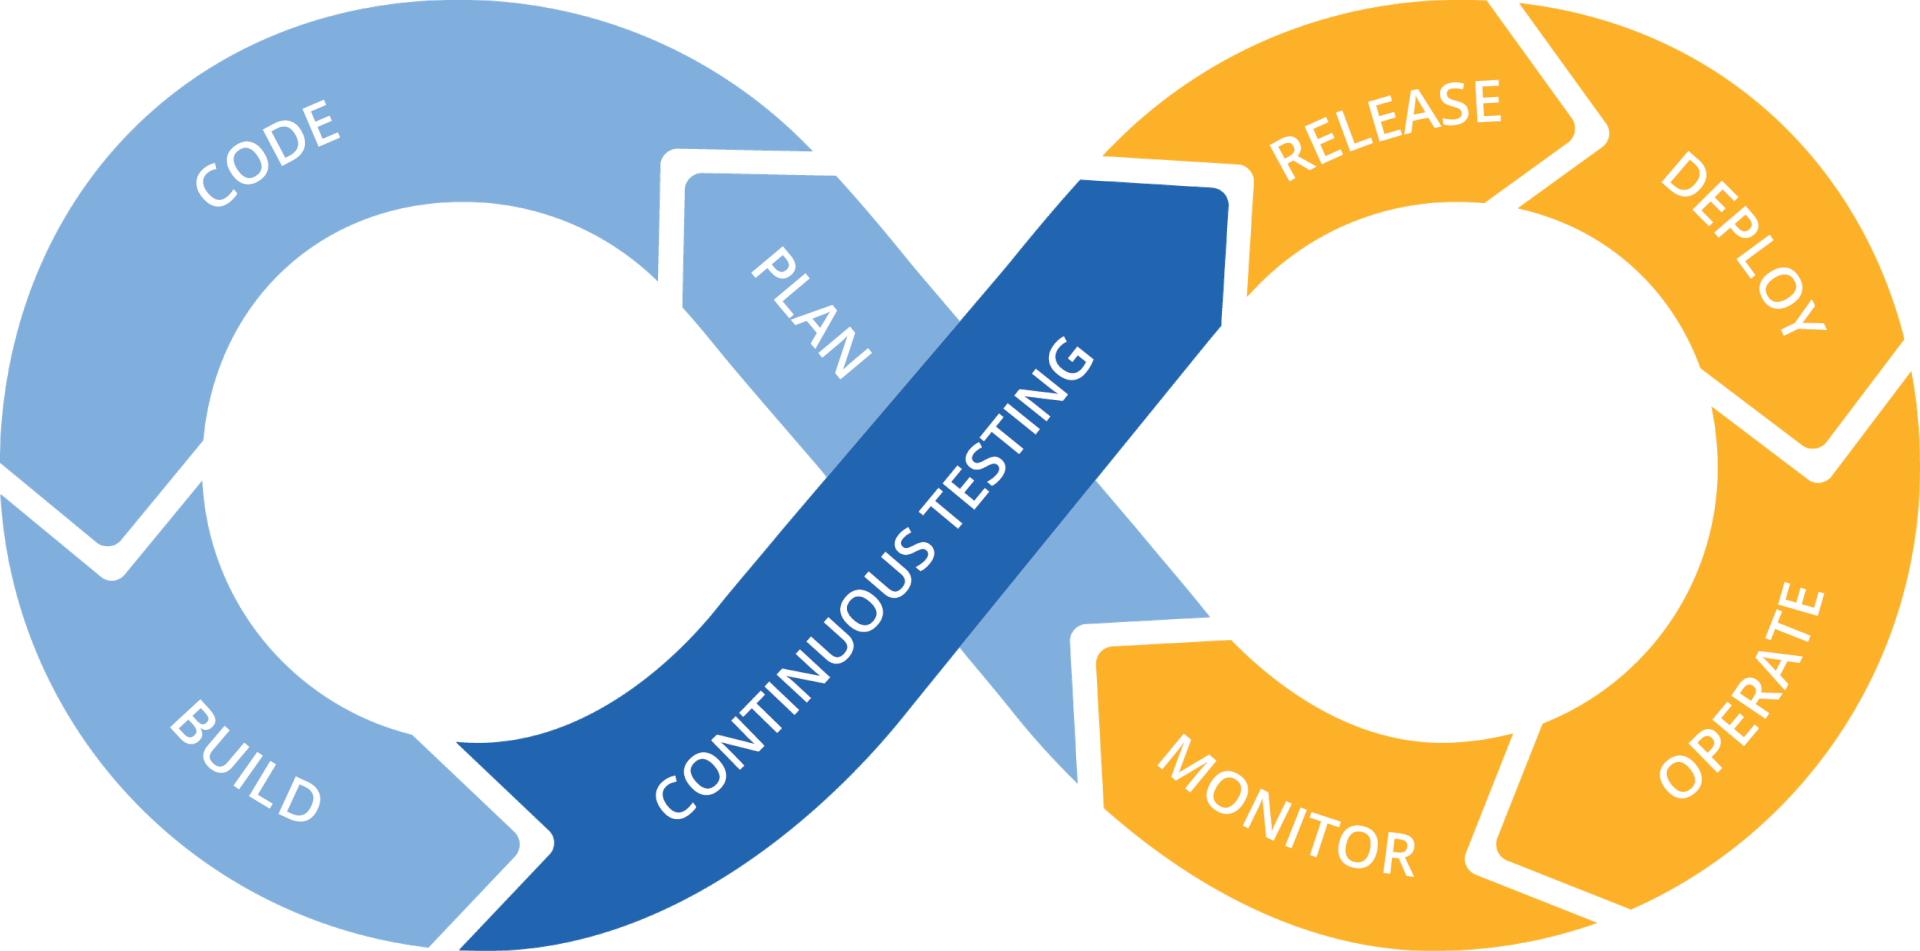
\includegraphics[width=0.5\textwidth]{Bilder/devopscycle}
	\caption{An example DevOpscycle}
	\label{fig:devopscycle}
\end{figure}
%\input{...further chapters...}
% !TeX spellcheck = en_US
 
\chapter{General Stack}
\label{chap:ch2}
\section{Collector}
To get Data in a centralized spot a tool is needed to collect the data were its generated and transport it to the Server or provide an Interface for the Server to collect the data.\\
Tools for this Purpose a we call Collectors. Were are Collector for every Monitoring Purpose. Its very common that a Collector provides a general interface like an XML or JSON data or can be adapted to variable Databases to get a wide spectrum of Use-Cases. The monitored metrics is dependent on the environment and the collector also has to use over tools that provides system data to get these type of metrics. In general the data that is collected can be split up in System data and Application data. System data are all physical values like CPU load, Ram and Hard Disc Drive usage.These will be providet by cAdvisor (\ref{cadvisor}) in the case of Kubernetes. Application data is dependent on the application. In the Case of monitoring Kubernetes normally the number of jobs/pods or the number of connection per time will be monitored. These and over data will be Providet by the Api-server(\ref{apiserver}) of Kubernetes.
\subsection{cAdvisor}
\label{cadvisor}
Container Advisor is tool for collection,Processing and Exporting Data of Containers. It is native Designed for Docker but can be applied to ever other container. All information about the Container is Accessible over a Rest api that gives back a JSON files with all data. A copy of cAdvisor is Deployed within every Kubernetes Pod, so every APM tool can get the metrics of the system.
\subsection{Api-Server}
\label{apiserver} 
Api-Server is a tool that provides a REST interface and is a front end for the hole Kubernetes Cluster. Over the Api-Server a user is able to interact with all Components of the cluster. The Api-Server also collects metrics witch are listed below.\\
\begin{itemize}
	\item Aggreation Controler Queue: Used for Parallel Processing as an Middelware
	\item Registration Controller:  
\end{itemize} 

\section{Database}
The Databases for a APM are usual time-series based (\ref{TS-Database}). As every other database its used to make data persistent and perform request over multiple entries to get new informations about critical values and value changes over time.
Databases can offer two types of data providing methods. Most of the time the database provides a well defined interface which normals provides a authentication method to insert data into the database. Every of these Snapshot than gets a timestamp.\\
The over method is that the database preforms a get operation onto a interface provided by the Collector. This type of data-collection is better for static system or must be 

\subsection{Time-Series-Database}
\label{TS-Database}
This is a special kind of database developed for saving time series data. This data consists of arrays which are indexed by a time stamp. By the term Time-Series also a time ranges cloud be used (as a primary key). These types of Databases  can create, enumerate, update, delete and analyze time-series-data.
Often they also allow you to merge multiple time-series together and make one.
Like each other database, time-series-databases can also filter the data which is normally order ascending by time.

\section{Visualization} 
The Visualization Tools are used to display the data stored in the databases in a nice and organized way. This is realized with plain text or by graphs. Graphs have the big advantage to be able to display the data changes over time and can very easily illustrate spikes in the data sets.Furthermore Graphs can present data in more than one way which makes it easier for humans to detect abnormal data spikes.\\
\\ 
Usually all this information can be accessed via a web interface as this also gives a nice option for logins and distribution of permissions. This is especially useful when the data is very sensitive.
Often these tools also implement easy to use Interfaces for Alerting tools, to set conditions for specific alerts, which can save a lot of time.

\subsection{Graphs}
As previously mentioned, the data we collected from the cluster needs to be written out of the Database and displayed in a nice and readable fashion. Thus most visualization tools use graphs to display the collected data. 
Using graphs not only makes the data easy to read, but it also adds the option to scale the data to our needs and preferences. This can be very useful when looking for trends in a bigger time range.\\
It also gives the option of color coding the data, which can be useful to either see dangerous values more quickly, or simply render multiple data streams in one graph to compare them or to see them im comparison too the hole system.
\subsection{Permission Management}
Most Visualization Tools have a web interface in which all the data is displayed. To make sure only authorized people can view the data, these tools usually implement a few permission management methods. 
These can be ranging from simple login permissions to viewing permissions of specific data streams. Some tools allow for complete customization of the permission settings, while others offer a set of permission templates. The most popular method of authorization seems to be LDAP, as this can be used for simple and complex permission schemes alike. 
\subsubsection{LDAP}
Written-out Lightweight Directory Access Protocol is a Network-protocol on a client-server basis. LDAP describes the communication between the client and the LDAP Directory. The data-structure of of LDAP is the so called Directory Information Tree which is organized by one suffix(root) and nodes.  
 


\section{Alerting}
To inform the developer about the system, a tool is needed which is able to sends warnings about predefined system states.
The alerting tool gets one or more error codes from the controller that is normally implemented into the database or visualization tool. Some tools combine With this codes the altering tool sends a warning or error message to all people involved. Most of the tools can send over multiple platforms. The most common are: E-Mail, SMS, telegram and slack. Often tools over man then the mentioned interface and provide a api to integrate other alerting types.\\
\\
Often the developers don’t want to get just one alert with one message, so some of the alerting tool have the possibility to sort the alerts into groups. With this feature its possible to group cascading events that are triggered by failure. In some cases tools also supply a option to divide all alerts into critical alerts and warnings which can help the user to select the important massages.  


%Hier wird der Hauptteil stehen. Falls mehrere Kapitel gewünscht, entweder mehrmals \texttt{\textbackslash{}chapter} benutzen oder pro Kapitel eine eigene Datei anlegen und \texttt{ausarbeitung.tex} anpassen.

%LaTeX-Hinweise stehen in \cref{chap:latextipps}.

%noch etwas Fülltext
\blinddocument

% !TeX spellcheck = en_US
 
\chapter{Tools} %Das ist nur ein Arbeitstitel
%\section{Template}
%\subsection{Toolname}
%\label{Toolname} % to refernce in the document
%Introduction Text with all infos about contributors 
%\subsection{Installation}
%Installation as we experienced it on the cluster
%\subsubsection{Appearance}%Only for Visual tools
%Description of the tool front-end with a Screen shot of the homepage/Dashboard
%\subsubsection{Performance}
%Quick analysis of the Performance (CPU/RAM usage during the test)
%\subsubsection{Interoperability}
%Which tools are listed to work with the tool/Which tools are test to work with the tool
%\subsubsection{Conclusion}
%A Quick Pro/Con of the tool and in which environment its best to use
\section{Searchlight (Icinga)}
\label{searchlight}
As in the section Icinga \ref{Icinga} described, we were not able to find a pure installation of Icinga for a cluster so we tried to install Searchlight as a backup plan.
Searchlight is a tool from the AppsCode Inc. (\url{https://appscode.com/},18.12.2017) which is a company located in San Leandro California. 
Searchlight is as many other monitoring tools written in the programming language of Go.
\\
When first trying this over the yaml File we received errors over the Kubernetes Cluster. There it says the tools is not able to bind the Port 8443. We could not figure out which application is using the port but as we tried to install the application on a fresh cluster VM it turns out the yaml deployment is working fine.
\subsection{Appearance}
%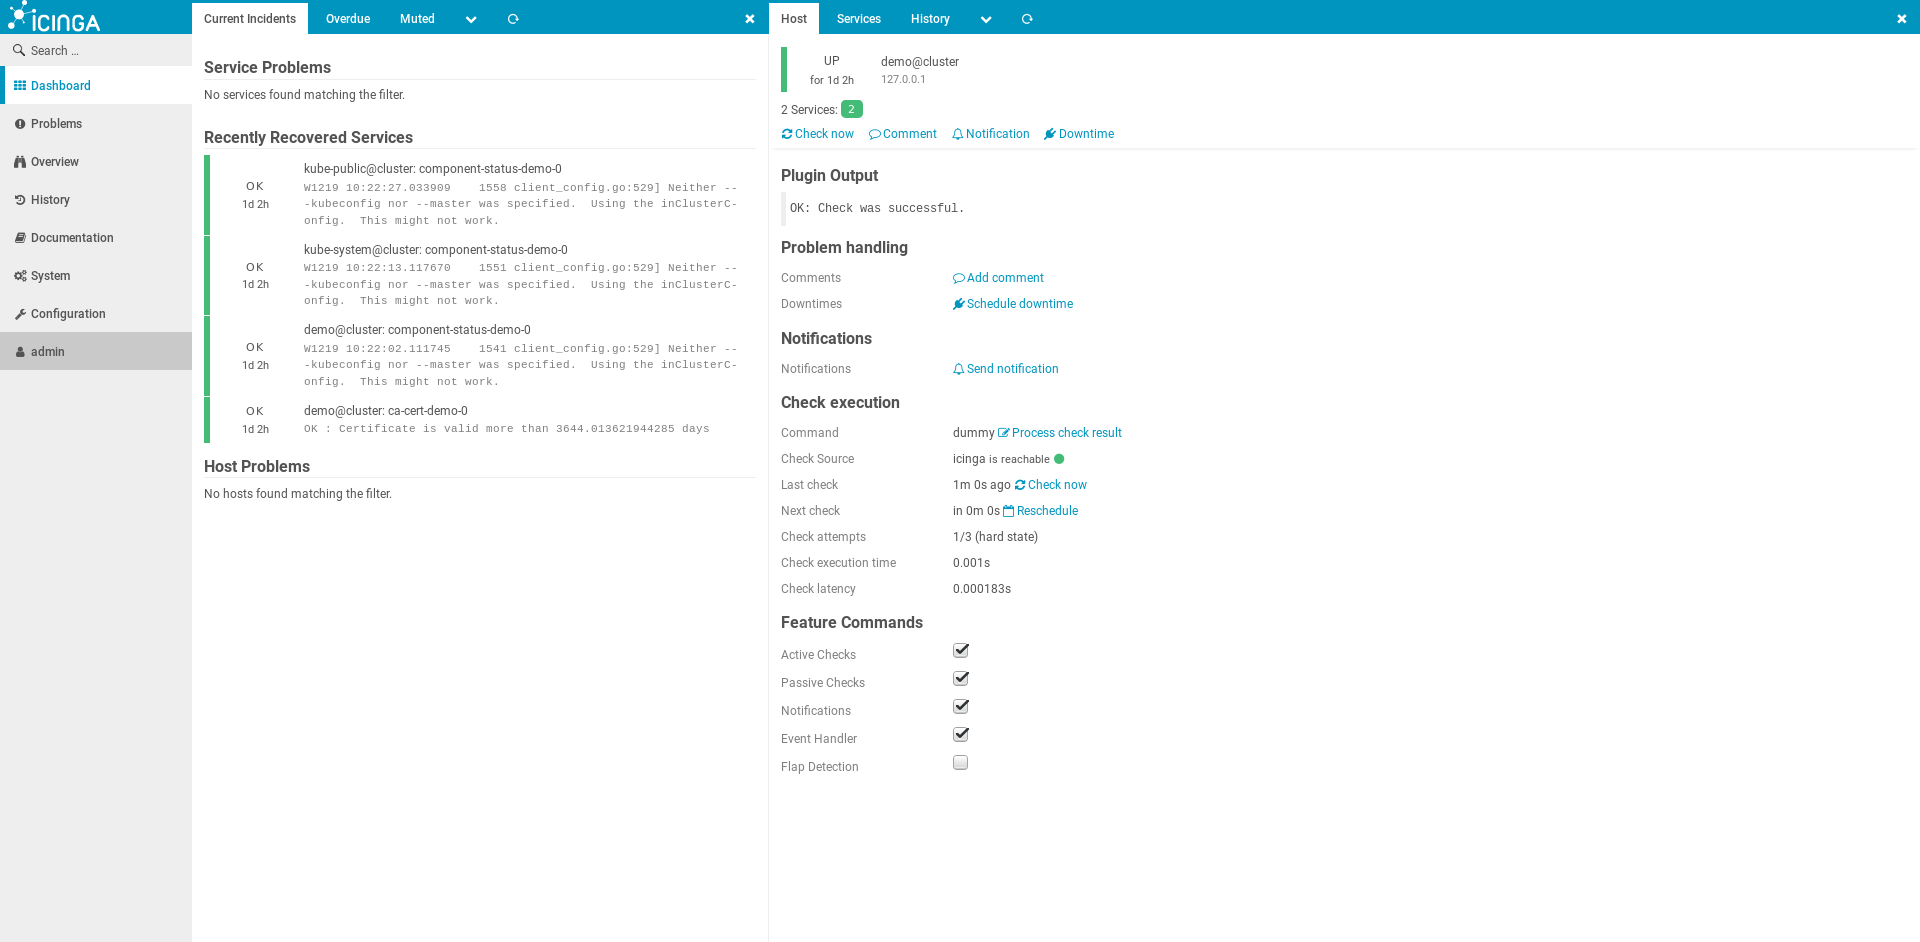
\includegraphics[width=1\linewidth]{Bilder/Searchlight_Icinga}\\
Icinga/Searchlight comes in a  discreet blue/withe coloring. On the Dashboard which represents the homepage of the application an overview of the implemented alerts is shown. The alerts will be colored with green/yellow/red for OK/warning/error, so its easy to see appearing problems. The rest of the options like History and Configurations is located at the sidebar. 
\subsection{Performance}
In our VM deployment the applications has allocated 160MB of RAM under load. The application it self is running very smooth even on low power systems. As we deployed some alerts we noticed that it took about 30 seconds to validate the alert and get a first status from the system. After that pending status everything is running smoothly and even checks on a 30 second rhythm were no problem for the system.
\subsection{Interoperability}
On the Github Page (\url{https://github.com/appscode/searchlight},20.12.2017) of the program the developer claims to be able to send notification over Email, SMS and Chat.
In the guide there is no explicit explanation what is meant by the term Chat but the tool is able to send notifications to Slack(\url{https://slack.com},03.01.2018) and Hipchat. Notification over Email can be send over SMTP without any third party software. To send SMS a service like Twilio(\url{https://www.twilio.com/},20.12.2017) is needed.
On the page there is no advise that the tool is capable to interact over an interface with other notification than the given. 
\subsection{Conclusion}
Searchlight is a light weighted  port of the famous monitoring tool Icinga. It runs well and has all basic needed features. On a deeper Look the software revealed its weakness. There are no advanced possibilities to connect Searchlight with over monitoring tools. Also there is no graphical user interface for creating alerts, which makes it very difficult to set it up. As the tool is manly only developed and updated by 2 two people the support for new versions of Icinga and Kubernetes is limited. The fact that the company Appcode has no direct correlation with Icinga is another counter-argument to the tool. In a nutshell the tool is good for small Kubernetes clusters that want to monitor only a few basic metrics and have low resources. 

\section{Prometeus}
\label{Prometeus} % to refernce in the document
The tool Prometeus is a open source project and is hosted by the Cloud Native Computing Foundation.
It is a single tool that comes with the features of a whole monitoring stack (without alerting).\\ Prometeus own collector uses client libraries, supported for different languages including GO, Java, Scala, Python and Ruby and more third-party libraries for various other languages. The Collector is able to pull data from the server or cluster and can be accessed via HTTP requests.\\
The project was originally built at Soundcloud and nowadays it is used by big companies like jodel, docker and Core OS (\url{https://prometheus.io/},20.0.1.2018). \\
Prometeus also has an alert manager, which is an extra tool to send message with the cluster state via E-Mail, HipChat, PagerDuty, Pushover, Slack, OpsGenie and VictorOps. These alerts have to be set up in an config file. \\
Because the project is community driven, there is no official repository for Kubernetes, but with a little research we managed to find this repository (https://github.com/kayrus/prometheus-kubernetes,10.01.2018) which provides different deployments for Kubernetes.

\subsection{Installation}
We managed to install Prometeus so that we were able to get metrics from the Api-server and can expose them over a restful interface. Over this interface it was possible to connect Prometeus to a application outside or inside the cluster like Grafana which is recommended for Prometeus. We were not able to install the Promteus own alertmanger on the cluster. Also we were not able to get metrics from the cluster-nodes because the Prometeus version is not cable of requesting over https. 
\subsection{Appearance}%Only for Visual tools
Prometeus provides a web user interface to see the collected data. It is designed in a very light wighted black and a with combination of some blue accents and it only shows the necessary things. The interface has no function to save the set of graphs that is selected and no option to login to keep the data save or to divide the data by some user groups.   
\subsection{Performance}
The tool is very quickly booted and shows no Performance problems on the interface. A look on the stats shows that Prometeus is not very CPU dependent, it oscillates up and down because the collection data peaks as show in \cref{fig:Prometeus_Cpu}. In the use of memory the tool is a little bit more demanding and takes up to 2GB of RAM. These high numbers of RAM is allocated over a time from about 24h. 
\begin{figure}
\centering
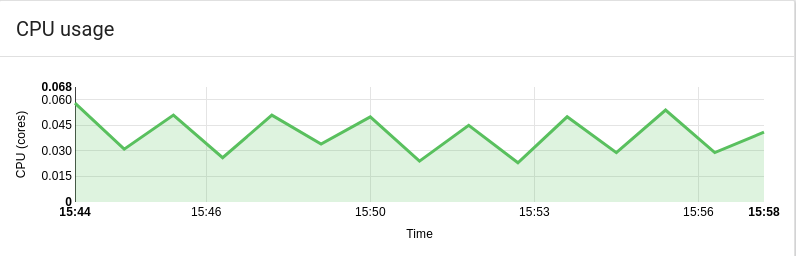
\includegraphics[width=0.7\linewidth]{Bilder/Performance/Prometeus_Cpu}
\caption{}
\label{fig:Prometeus_Cpu}
\end{figure}
\subsection{Interoperability}
It's highly recommended that Prometeus is used with a graphing and alerting tool because its just a collector and time series database with a query engine. In our deployment Graphana is used, which is also recommended by the Prometeus web page (\url{https://prometheus.io/},12.01.2018). Exploiting Prometheus to any other tool is also possible as Prometeus provides the metrics that are collected in plain text
\subsection{Conclusion}
Prometeus is very good as a collector for large Kubernetes Clusters with hundreds or thousands of nodes. What makes it so good is the with-box monitoring approach, which provides way more metrics than a black-box monitoring. These fact can be used to detect problems in the system earlier and in much more detail so that the downtime can be reduced. On the other side Prometeus is not good for presenting this data and to throw alerts in case of failure.

\section{Zabbix}
\label{Zabbix} % to refernce in the document
% \url{https://dl.acm.org/citation.cfm?id=1883485} Linux Journal
\cite{Hernantes2015}
The tool Zabbix is an open-source tool and is developed by Zabbix LLC (Limited Liability Company) since 2005 (\url{https://www.zabbix.com},15.01.2018). Zabbix provides a all in one Solution with includes a Collector, Database, Visualization tool and a alert manager. Moreover there is a repository from monitoringartist (\url{https://github.com/monitoringartist/kubernetes-zabbix},15.01.2018) that provides a yaml which maps Zabbix client and server on a cluster structure.  
\subsection{Appearance}%Only for Visual tools
Zabbix come with a withe and blue web interface with some red accents. It implements a tab system with subtabs to navigate through the interface. The naming of the tabs is not as self explaining as it could be.  
\subsection{Performance}
The general performance of Zabbix is very good. The three parts take up to 1GB of RAM of the System and about 0.5 \% of the processor load. The Minimum requirements of Zabbix are specified with Pentium 2 of 350Mhz and 256MB of Ram \cite{Marik2014}.
\subsection{Interoperability}
Zabbix provides a different API to connect to other entities. The web interface  provide a PHP script that accepts queries. Grafana itself has a extra plug in which is connectible to Zabbix and show a optimized dashboard with all relevant informations. The tool is also capable of sending alerts over email, SMS, and jabber. Zabbix gives also the ability to create customscripts and to execute them in case of a alert. For example a cli script can be triggerd over ssh. 
\subsection{Conclusion}
Zabbix is one of the best optimized and extended open-source solutions available. The installation was by far the simplest and overarching of all the tested tools. The configuration is complex and the naming is not at ever position as aspected. By default Zabbix scales over all of the available nodes but can be scaled up manual. The best way to use Zabbix is to pare it with a Grafana instance which provides the information from Zabbix tighter and with a better overview.

\section{ELK Stack (logstash, elasticsearch, kibana)}
\label{elk} % to refernce in the document
Elasticsearch is a tool developed by elastic.(\url{https://www.elastic.co/}, 10.01.2018) The company Elastic has many locations all around the world and seems to be very present for its customers.
The ELK Stack is a logging tool which is developed java and divided up into three parts. First the logstash, the Collector of the stack. Second elasticsearch which queries the data given by the collector and last kibana the visualization tool of the stack.
\subsection{Installation}
ELK Stack is deployable at the kubernetes cluster. There is a solution on github provided by kubernetes. After the installation there 
\subsection{Appearance}%Only for Visual tools
Kibana is the only tool in the complete Stack with a user interface. It is accessible over the homepage of the application. The site is starting with a discover page, where all logs are listed in a time chronological order. The discover page also allows to filter these logs by key words. On the leftside is the sidebar with management, devtools, visualize, timeline, discoverer and dashboard. The dashboard tab, is for creating an own dashboard with the own preferences.
\subsection{Performance}
Quick analysis of the Performance (CPU/RAM usage during the test)
\subsection{Interoperability}
Elasticsearch also offers many a tool to include alerts. The tool can send any alerts which you can query with elasticsearch. On the official website, elastics mentioned they can send the notifications on E-Mail, PagerDuty, Slack and HipChat and it also offers an interface with an webhook-output to integrate any third-party-software for messaging. With this interface it might be easy to include sending alerts with SMS like earlier mentioned the program Twilio(\ref{searchlight}).
\subsection{Conclusion}
A Quick Pro/Con of the tool and in which environment its best to use

\section{Grafana}
\label{grafana} % to refernce in the document
Grafana is a tool to visualize the data collected about a system. It features different graphs, including graphs with changes over time, single stats for live feeds, tables to show multiple data from different sources and heatmaps to show the distribution of values over a timespan.
Grafana also comes with an inbuilt alerting system which allows the user to be notified under specific conditions via E-Mail, Slack, PagerDuty, DingDing / DingTalk, Kafka. The alerting also has a webhook, allowing the user to send his alerts to a custom endpoint via HTTP.
The graphs and alerts are setup in the web interface of Grafana which comes with its own user management. It differentiates between users and administrators and super-administrators. Administrators can be assigned to an organization, allowing different systems to be monitored by one Grafana instance, while still giving the owners of the single system the option to manage their own alerts and graphs.
Grafana also features a LDAP Authentication to automatically import users and permissions from a user directory.
\subsection{Installation}
The installation of Grafana is very simple, because it only runs on a single Docker container. Because Grafana is no collector over tools provide an extra version of Grafana in there repository that is optimized for there data sources.
\subsection{Appearance}%Only for Visual tools
Grafana mainly uses the colors red and orange and comes with a dashboard. Due to the data source that is selected this changes to a set of graphs which show the information of the data source. Per drag and drop the graphs and text boxed can be freely moved around. 
\subsection{Performance}
The performance of Grafana is very good. The tools consumes nearly no CPU and only a few megabytes of RAM as shown in \cref{fig:Grafan_RAM}. The Diagram also shows that the amount of the used resources is constant over time
\begin{figure}
\centering
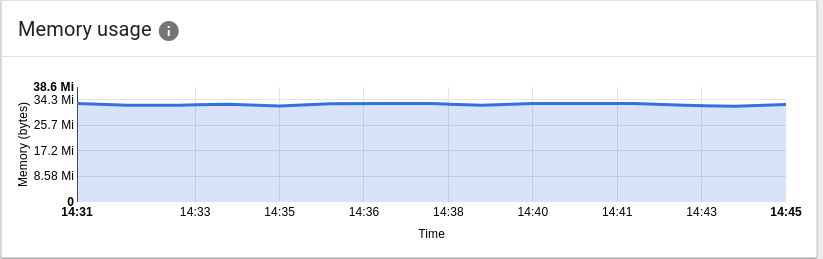
\includegraphics[width=\textwidth]{Bilder/Performance/Grafan_RAM}
\caption{Graphane Ressource use}
\label{fig:Grafan_RAM}
\end{figure}
\subsection{Interoperability}
Grafana can interact with nearly every interface to sent alerts because of its Web hooks which can send and request to an restful endpoint over a JSON document. Whats special about the alerting engine of Grafana is that pictures can be send within the alerts. The pictures is taken of the Grafana to present the alert in a visual way and can be send with the notification or can be uploaded to services like Amazon S3.

\subsection{Conclusion}
Grafana is by far the best and biggest visualization tool on the open-source market. Due to the capability to write custom plugins nearly every tool stack has an integration which is easy to install and uses the features of Grafana in the intention of the developer.

\section{Failed Tools}%Ebenfalls nur ein arbeitstitel
In the process of developing and evaluating the APM we discovered a bunch of tools that we were not able to install even that they claimed to be optimized to work on Kubernetes .
In this paragraph all the tools we wanted to include in our report but doesn't work, are mentioned with a quick description of the failure.
\subsection{Graphite}
Graphite is mainly for storing and graphing data and metrics, but brings also tools that are able to collect these metrics from the system. By the developer it self there is no Kubernetes installation provided but there are diverse approaches by third party members to make it runnable on a Cluster. We have tested the Repository from nanit\\(\url{ https://github.com/nanit/kubernetes-graphite-cluster},11.12.2017) to get Graphite running with StatsD (\url{https://github.com/etsy/statsd.git},11.12.2017) as a metric collection tool. The Repository doesn't provide a yaml file by it self to install all the tools. The instruction leads the user to export some variables needed for the installation. After that a deploy command is provided that pulls the docker repository and than installs it with kubectl on the Cluster. As we tried to execute this command an error was thrown, The node replicas were empty, so no further commands are executable. As we were not able to install the tool on multiple Kubernetes Clusters, we installed the tool as on the website advertised on a Ubuntu system directly. With this installation of Graphit a time-series data, an monitoring and alerting tool is included. On the test system the monitoring system gave values that differs from the Linux intern monitoring in values like CPU usage or RAM. As a solution to all this difficulties we decided to not perform further test on the tool.

\subsection{Icinga}
\label{Icinga}
Icinga is as ELK-Stack not a monitoring tool. Its made for logging defined requests. The administrator can decide which system to monitor and in what interval the data is pulled.
Icinga it self only provides 3 system states instead of exact values. The states are OK/warning and error. The user decides at which point they are triggered.\\
As we tried to install Icinga we found out that there was no direct support from Incinga for Kubernetes. As our Study only describes the actual state without trying to add something we decided not to try an compile Icinga into Kuberntes on our own. Later we found out there is a third party Software called searchlight \ref{searchlight} which is provided by appscode on github.
 
% !TeX spellcheck = en_US
\chapter{Evaluation} %Das ist nur ein Arbeitstitel
% \useunder{\uline}{\ul}{}
This chapter deals with the comparison of the tools grouped by their responsibility. First, we explain some concepts, we have encountered in our research. These concepts will be covered in \cref{concepts}.
Each table shows the specification the developer gives. They are ordered by the responsibility of tools. The information shown in the tables are from the website of the tool providers.
In all tables below we indicated present features with a $ \checkmark $ and non-present features with a $ x $, if they were advertised by the developer.
\section{Comparison of concepts}
\label{concepts}
In the scope of this study we identified concepts to group the tools by comparison. Most of them are self explanatory. The ones that are not self explanatory are listed below with a brief introduction.
\subsection{Push/Pull}
\label{push/pull}
There are two basic concepts of the exchange of informations between the collector and the database. Hereby referred as push and pull. Push \cite{5557986} is a concept, were the collector  automatically starts sending data to the database as soon the system is started. The data is send continuously. Important is that the collector knows or discovers the data destination, mostly through the use of a discoverer.
Pull \cite{5557986} on the other hand means that the database sends requests to all active nodes. These requests are executed in certain intervals. These intervals can be modified and adjusted according to the system requirements. In this concept the database needs a discoverer to find all existing nodes
\subsection{REST}
\label{rest}
Representational State Transfer is a programming paradigm for distributed systems. It describes a way, how services in special web services interact with each other. Important concepts of REST are loose coupling, interoperability and scalability. Any data in REST is made persistent in resources. These resources are addressable over an Uniform Resource Identifier. \\
To make an interface RESTful, it has to provide all HTTP methods like GET, PUT, POST, OPTIONS within a well known data format as XML or JSON \cite{rest}.


\section{Collector}
The \cref{tab:Collector} compares the different collector tools tested in this paper. The tools are compared by RESTful (\cref{rest}), Multiple(Multi.) Input Formats, Plug-ins for own data and Push/Pull (\cref{push/pull}).
\begin{table}[H]
\centering
\begin{tabular}{lcccc}
\hline

Tool & RESTful & Multi. Input Formats      & Plug-ins for own data        & Push / Pull \\

\hline
Telegraf    & Yes ($ \checkmark $) & Yes    & Yes    &Pull    ($ \checkmark $)  \\
Beats  & Yes ($ \checkmark $)  & Yes & Yes  & Push ($ \checkmark $) \\
Logstash & Yes ($ \checkmark $)  & No & Yes & Push/Pull($\checkmark$)                         \\
Icinga2  & No  & No  & Yes  & Push \\
Prometheus  & No  & No  & Yes  & Pull ($ \checkmark $)/ Push\\
Zabbix & No  & No  & No  & Both \\
\hline                        
\end{tabular}
\caption{Collector-table - All tested collector tools are listed and compared}
\label{tab:Collector}
\end{table}

\section{Database}
\cref{tab:Database} shows the databases. First we checked if the tools have an authentication-based asses to  the content. Furthermore we have selected the tools according to time-series-database. In addition to that, we checked, if multiple datasets per time stamp are allowed. 
\begin{table}[H]
\centering
\begin{tabular}{lccc}
	\hline
Tool & Database-Authentication     & Time-Series-Database          & Multi. Data Points        \\
\hline
InfluxDB  & Yes ($ \checkmark $) & Yes ($ \checkmark $)  & Yes ($ \checkmark $)\\
Elasticsearch & https ($ \checkmark $), credentials ($ X $) & Yes ($ \checkmark $) & Yes ($ \checkmark $)\\
Icinga2 & Yes ($ \checkmark $) & Yes ($ \checkmark $) & Yes ($ \checkmark $) \\
Prometheus& No & Yes ($ \checkmark $) & Yes ($ \checkmark $)\\
Zabbix& Yes ($ \checkmark $) & Yes ($ \checkmark $) & Yes ($ \checkmark $)\\
\hline
\end{tabular}
\caption{Database-table - All tested database tools are listed and compared}
\label{tab:Database}
\end{table}

\section{Visualization}
\cref{tab:Visualization} compares the different visualization tools. One aspect is the security of the tool, this is compared by LDAP-Authentication (\cref{ldap}). In general the tools are tested on the base of the graphs that they can display. We tested if they are scalable and whether or not it is possible to show multiple graphs in one. 
\begin{table}[H] 
\centering
\begin{tabular}{lccc}
	\hline
Tool & LDAP-Authentication         & Scalable graphs             & Overlapping graphs          \\
\hline
Chronograf & No & Yes & Yes \\
Kibana & Yes ($ \checkmark $) & Yes ($ \checkmark $) & Yes ($ \checkmark $)\\
Grafana & Yes ($ \checkmark $) & Yes ($ \checkmark $) & Yes ($ \checkmark $)\\
Zabbix & Yes ($ \checkmark $) & Yes ($ \checkmark $)  & Yes  ($ \checkmark $)\\
\hline
\end{tabular}
\caption{Visualization-table - All tested visualization tools are listed and compared}
\label{tab:Visualization}
\end{table}

\section{Alerting}
The last two tables (\cref{tab:Alerting}) and (\cref{tab:Alertingcont}) compares the altering tools. These tools were tested if they can send HTTP requests. Moreover, when many identical alerts arrive, whether they are groupable. Furthermore we tested the most common messaging tools for sending alerts and if the tools offer an interface to integrate any third-party-tool for messaging. Finally, the tools have been tested for triggering events like scripts when an alert is received.
\begin{table}[H]
	\centering
	\begin{tabular}{lcccc}
		\hline
Tool & HTTP requests & Grouping of alerts & E-Mail & Messangers \\
\hline
Kapacitor & Yes  & No & Yes & Yes \\
Elastalert & No & No & Yes ($ \checkmark $) & Yes ($ \checkmark $) \\
Grafana & Yes ($ \checkmark $) & Yes ($ \checkmark $) & Yes ($ \checkmark $) & Yes ($ \checkmark $) \\
Zabbix & Yes ($ \checkmark $) & Yes ($ \checkmark $) & Yes ($ \checkmark $) & Yes ($ \checkmark $) \\
Prometheus & Yes ($ \checkmark $) & Yes ($ X $) & Yes ($ X $) & Yes ($ X $)\\
		\hline
	\end{tabular}
	\caption{Alerting-table - All tested alerting tools are listed and compared}
	\label{tab:Alerting}
\end{table}

% Please add the following required packages to your document preamble:
% \usepackage[table,xcdraw]{xcolor}
% If you use beamer only pass "xcolor=table" option, i.e. \documentclass[xcolor=table]{beamer}
\begin{table}[H]
	\centering
	\begin{tabular}{lcc}
		\hline
		Tool & Custom alerts & Action on alert \\
		\hline
		Kapacitor                    & Yes ($ \checkmark $)       & No\\
		Elastalert                   & Yes ($ \checkmark $) & No\\
		Grafana                      & Yes ($ \checkmark $)          & Yes ($ \checkmark $)\\
		Zabbix  & Yes ($ \checkmark $) & Yes ($ \checkmark $)\\
		Prometheus & Yes ($ \checkmark $) & No \\
		\hline 
	\end{tabular}
	\caption{Alerting-table - \cref{tab:Alerting} cont.}
	\label{tab:Alertingcont}
\end{table}


% !TeX spellcheck = en_US

\chapter{Conclusion}\label{chap:conclusion}
\section{General Trends}
Most of the systems we evaluated or considered evaluating were metric monitoring stacks. In general most tools detect not the cause of the failure. Instead the effect is recognized and can be treated manual. With some tools we saw a trend towards more automation. These tools had functions like automated script triggering over ssh or automatic delivery of logs in the alert message. \\
\\
Another trend is that alerting manager implement a massive amount of different services for messaging that are used by modern developer teams like slack or telegram. Some of the bigger tools were also capable of REST or SOAP requests so that nearly every interface can be included. To keep overview of cascading failure ,some of the tools can group errors to one alert.
\\
In Visualization a big trend is the presentation of similar data in one single graph. These method provides a better overview of the system and leads to generalization of the data. Moreover the most tools use coloring to highlight warnings or errors. The big player on the market also implement a custom ordering engine, to drag around the graphs for an own sorting.
\\
We also saw some tendency in the database evolution. Databases are no longer just for storing single data points. They now have a greater added value by implementing there own querying language. Using this to purify the collected the data for visualization tools. The most established data format is JSON because the files can be fragmented over multiple nodes.

The field of collectors drifts towards multi functional interfaces. These trend is settled, because many system have to be integrated in already existing monitoring environments. In addition there are two types of collectors. Once the log collectors and secondly the metric one's. Both are necessary to monitor a complete system as a whole.

When we installed and tested the tools, all of the above trends were reflected in them. That is how we identified and worked out the trends. 


%With a more deeper look in the logging monitoring tools some more trends of the different tool types could be found and identified. 
\section{Conclusion}
At the beginning of this paper we asked the question which monitoring tools are the best. Clear is that there is no clear answer to this question. It always depends on the environment that is used, often some monitoring structure is already given and a new solutions have to be build around them.\\
To answer the question anyway we decided to recommend an combination from Zabbix and Grafana for Kubernetes monitoring. We think it is good, because the installation is very easy and can be done with one single command line. There are also different versions of the Zabbix portation. Some of them are more lightweighted or have more tools than the others. In terms of functions Zabbix nearly provides everything. To complete this functionality with usability and interoperability we recommend to configure a Grafana instance onto the REST api of Zabbix. This is easy done because Grafana has it own Zabbix plug-in. This plug-in provides a very nice dashboard view of the cluster metrics.
%TO DO
\\
If there is any reason to not go for an Zabbix installation or if a deeper look into the single nodes and pods is required, we could recommend a combination of Heapster with Influxdb and Grafana. The installation is a little bit more complex because all the tools have to be configured to work together. The huge benefit is that all tools are adopted by the Kubernetes Developers to work great with the cluster. This not only allows a very detailed look on every Pod that is deployed. The tools also offer a great performance even in small clusters. In special the Ram usage was lower than of any other tested tools.

\section*{Future Work}
As a follow up to our work a deeper look into the field of log monitoring tools could provide a more efficient way of failure treatment. An important task to look is where micro service environments like Kubernetes or technology like docker store there logs. To get the best benefit out of the logs it is a major task to find a good storing engine for the quickly changing services. We think a clear mapping of the logs to the service informations is a main quest of the work.\\
As we only looked at solutions that are open-source there is the possibility to expand our work to the hole software market to take more tools into account. This work could discuss the question of benefits that open source has over paid tools for the new DevOps style of developing.


%
%
%\renewcommand{\appendixtocname}{Anhang}
%\renewcommand{\appendixname}{Anhang}
%\renewcommand{\appendixpagename}{Anhang}
\appendix
%% !TeX spellcheck = de_DE
%Die Angabe des schlauen Spruchs auf diesem Wege funtioniert nur,
%wenn keine Änderung des Kapitels mittels den in preambel/chapterheads.tex
%vorgeschlagenen Möglichkeiten durchgeführt wurde.
\setchapterpreamble[u]{%
\dictum[Albert Einstein]{Probleme kann man niemals mit derselben Denkweise lösen, durch die sie entstanden sind.}
}
\chapter{LaTeX-Tipps}
\label{chap:latextipps}

\section{File-Encoding und Unterstützung von Umlauten}
\label{sec:firstsectioninlatexhints}
Die Vorlage wurde 2010 auf UTF-8 umgestellt.
Alle neueren Editoren sollten damit keine Schwierigkeiten haben.

\section{Zitate}
Referenzen werden mittels \texttt{\textbackslash cite[key]} gesetzt.
Beispiel: \cite{WSPA} oder mit Autorenangabe: \citet{WSPA}.

Der folgende Satz demonstriert \begin{inparaenum}[1.]
\item die Großschreibung von Autorennamen am Satzanfang,
\item die richtige Zitation unter Verwendung von Autorennamen und der Referenz,
\item dass die Autorennamen ein Hyperlink auf das Literaturverzeichnis sind sowie
\item dass in dem Literaturverzeichnis der Namenspräfix \enquote{van der} von \enquote{Wil M.\,P.\ van der Aalst} steht.
\end{inparaenum}
\Citet{RVvdA2016} präsentieren eine Studie über die Effektivität von Workflow-Management-Systemen.

Der folgende Satz demonstriert, dass man mittels \texttt{label} in einem Bibliopgrahie"=Eintrag den Textteil des generierten Labels überschreiben kann, aber das Jahr und die Eindeutigkeit noch von biber generiert wird.
Die Apache ODE Engine \cite{ApacheODE} ist eine Workflow-Maschine, die BPEL-Prozesse zuverlässig ausführt.

Wörter am besten mittels \texttt{\textbackslash enquote\{...\}} \enquote{einschließen}, dann werden die richtigen Anführungszeichen verwendet.

Beim Erstellen der Bibtex-Datei wird empfohlen darauf zu achten, dass die DOI aufgeführt wird.

\section{Mathematische Formeln}
\label{sec:mf}
Mathematische Formeln kann man $so$ setzen. \texttt{symbols-a4.pdf} (zu finden auf \url{http://www.ctan.org/tex-archive/info/symbols/comprehensive/symbols-a4.pdf}) enthält eine Liste der unter LaTeX direkt verfügbaren Symbole.
Z.\,B.\ $\mathbb{N}$ für die Menge der natürlichen Zahlen.
Für eine vollständige Dokumentation für mathematischen Formelsatz sollte die Dokumentation zu \texttt{amsmath}, \url{ftp://ftp.ams.org/pub/tex/doc/amsmath/} gelesen werden.

Folgende Gleichung erhält keine Nummer, da \texttt{\textbackslash equation*} verwendet wurde.
\begin{equation*}
x = y
\end{equation*}

Die Gleichung~\ref{eq:test} erhält eine Nummer:
\begin{equation}
\label{eq:test}
x = y
\end{equation}

Eine ausführliche Anleitung zum Mathematikmodus von LaTeX findet sich in \url{http://www.ctan.org/tex-archive/help/Catalogue/entries/voss-mathmode.html}.

\section{Quellcode}
\Cref{lst:ListingANDlstlisting} zeigt, wie man Programmlistings einbindet.
Mittels \texttt{\textbackslash lstinputlisting} kann man den Inhalt direkt aus Dateien lesen.

%Listing-Umgebung wurde durch \newfloat{Listing} definiert
\begin{Listing}
\begin{lstlisting}
<listing name="second sample">
  <content>not interesting</content>
</listing>
\end{lstlisting}
\caption{lstlisting in einer Listings-Umgebung, damit das Listing durch Balken abgetrennt ist}
\label{lst:ListingANDlstlisting}
\end{Listing}

Quellcode im \lstinline|<listing />| ist auch möglich.

\section{Abbildungen}

Die \cref{fig:chor1} und \ref{fig:chor2} sind für das Verständnis dieses Dokuments wichtig.
Im Anhang zeigt \vref{fig:AnhangsChor} erneut die komplette Choreographie.

%Die Parameter in eckigen Klammern sind optionale Parameter - z.B. [htb!]
%htb! bedeutet: "Liebes LaTeX, bitte platziere diese Abbildung zuerst hier ("_h_ere"). Falls das nicht funktioniert, dann bitte oben auf der Seite ("_t_op"). Und falls das nicht geht, bitte unten auf der Seite ("_b_ottom"). Und bitte, bitte bevorzuge hier und oben, auch wenn's net so optimal aussieht ("!")
%Diese sollten nach Möglichkeit NICHT verwendet werden. LaTeX's Algorithmus für das Platzieren der Gleitumgebung ist schon sehr gut!
\begin{figure}
  \centering
  \includegraphics[width=\textwidth]{choreography.pdf}
  \caption{Beispiel-Choreographie}
  \label{fig:chor1}
\end{figure}

\begin{figure}
  \centering
  \includegraphics[width=.8\textwidth]{choreography.pdf}
  \caption[Beispiel-Choreographie]{Die Beispiel-Choreographie. Nun etwas kleiner, damit \texttt{\textbackslash textwidth} demonstriert wird. Und auch die Verwendung von alternativen Bildunterschriften für das Verzeichnis der Abbildungen. Letzteres ist allerdings nur Bedingt zu empfehlen, denn wer liest schon so viel Text unter einem Bild? Oder ist es einfach nur Stilsache?}
  \label{fig:chor2}
\end{figure}


\begin{figure}
  \centering
    \subfloat[]{\includegraphics[width=0.3\textwidth]{choreography.pdf} \label{fig:subfigA}}
    \subfloat[]{\includegraphics[width=0.3\textwidth]{choreography.pdf} \label{fig:subfigB}}
		\subfloat[Subcaption if needed]{\includegraphics[width=0.3\textwidth]{choreography.pdf} \label{fig:subfigC}}
	\caption{Beispiel um 3 Abbildung nebeneinader zu stellen nur jedes einzeln referenzieren zu können. Abbildung~\ref{fig:subfigB}
 ist die mittlere Abbildung.}
\label{fig:subfig_example}
\end{figure}

Das SVG in \cref{fig:directSVG} ist direkt eingebunden, während der Text im SVG in \cref{fig:latexSVG} mittels pdflatex gesetzt ist.
\todo{Falls man die Graphiken sehen möchte, muss inkscape im PATH sein und im Tex-Quelltext \texttt{\textbackslash{}iffalse} und \texttt{\textbackslash{}iftrue} auskommentiert sein.}

\iffalse % <-- Das hier wegnehmen, falls inkscape im Pfad ist
\begin{figure}
\centering
\includegraphics{svgexample.svg}
\caption{SVG direkt eingebunden}
\label{fig:directSVG}
\end{figure}

\begin{figure}
\centering
\def\svgwidth{.4\textwidth}
\includesvg{svgexample}
\caption{Text im SVG mittels \LaTeX{} gesetzt}
\label{fig:latexSVG}
\end{figure}
\fi % <-- Das hier wegnehmen, falls inkscape im Pfad ist

\section{Tabellen}

\cref{tab:Ergebnisse} zeigt Ergebnisse und die \cref{tab:Ergebnisse} zeigt wie numerische Daten in einer Tabelle representiert werden können.
\begin{table}
  \centering
  \begin{tabular}{ccc}
  \toprule
  \multicolumn{2}{c}{\textbf{zusammengefasst}} & \textbf{Titel} \\ \midrule
  Tabelle & wie & in \\
  \url{tabsatz.pdf}& empfohlen & gesetzt\\

  \multirow{2}{*}{Beispiel} & \multicolumn{2}{c}{ein schönes Beispiel}\\
   & \multicolumn{2}{c}{für die Verwendung von \enquote{multirow}}\\
  \bottomrule
  \end{tabular}
  \caption[Beispieltabelle]{Beispieltabelle -- siehe \url{http://www.ctan.org/tex-archive/info/german/tabsatz/}}
  \label{tab:Ergebnisse}
\end{table}

\begin{table}
	\centering
	\begin{tabular}{l *{8}{d{3.2}}}
		\toprule
						
			   & \multicolumn{2}{c}{\textbf{Parameter 1}} & \multicolumn{2}{c}{\textbf{Parameter 2}} & \multicolumn{2}{c}{\textbf{Parameter 3}} & \multicolumn{2}{c}{\textbf{Parameter 4}} \\
			\cmidrule(r){2-3}\cmidrule(lr){4-5}\cmidrule(lr){6-7}\cmidrule(l){8-9}
			
			\textbf{Bedingungen} & \multicolumn{1}{c}{\textbf{M}} & \multicolumn{1}{c}{\textbf{SD}} & \multicolumn{1}{c}{\textbf{M}} & \multicolumn{1}{c}{\textbf{SD}} & \multicolumn{1}{c}{\textbf{M}} & \multicolumn{1}{c}{\textbf{SD}} & \multicolumn{1}{c}{\textbf{M}} & \multicolumn{1}{c}{\textbf{SD}}\\
			\midrule
			
			W & 1.1 & 5.55 & 6.66 & .01 &  &  &  & \\
			X & 22.22 & 0.0 & 77.5 & .1 &  &  &  & \\
			Y & 333.3 & .1 & 11.11 & .05 &  &  &  & \\
			Z & 4444.44 & 77.77 & 14.06 & .3 &  &  &  & \\
		\bottomrule 
	\end{tabular}
	
	\caption{Beispieltabelle f\"{u}r 4 Bedingungen (W-Z) mit jeweils 4 Parameters mit (M und SD). Hinweiß: immer die selbe anzahl an Nachkommastellen angeben.}
	\label{tab:Werte}
\end{table}

\section{Pseudocode}
\Cref{alg:sample} zeigt einen Beispielalgorithmus.
\begin{Algorithmus} %Die Umgebung nur benutzen, wenn man den Algorithmus ähnlich wie Graphiken von TeX platzieren lassen möchte
\caption{Sample algorithm}
\label{alg:sample}
\begin{algorithmic}
\Procedure{Sample}{$a$,$v_e$}
\State $\mathsf{parentHandled} \gets (a = \mathsf{process}) \lor \mathsf{visited}(a'), (a',c,a) \in \mathsf{HR}$
\State \Comment $(a',c'a) \in \mathsf{HR}$ denotes that $a'$ is the parent of $a$
\If{$\mathsf{parentHandled}\,\land(\mathcal{L}_\mathit{in}(a)=\emptyset\,\lor\,\forall l \in \mathcal{L}_\mathit{in}(a): \mathsf{visited}(l))$}
\State $\mathsf{visited}(a) \gets \text{true}$
\State $\mathsf{writes}_\circ(a,v_e) \gets
\begin{cases}
\mathsf{joinLinks}(a,v_e) & \abs{\mathcal{L}_\mathit{in}(a)} > 0\\
\mathsf{writes}_\circ(p,v_e)
& \exists p: (p,c,a) \in \mathsf{HR}\\
(\emptyset, \emptyset, \emptyset, false) & \text{otherwise}
\end{cases}
$
\If{$a\in\mathcal{A}_\mathit{basic}$}
  \State \Call{HandleBasicActivity}{$a$,$v_e$}
\ElsIf{$a\in\mathcal{A}_\mathit{flow}$}
  \State \Call{HandleFlow}{$a$,$v_e$}
\ElsIf{$a = \mathsf{process}$} \Comment Directly handle the contained activity
  \State \Call{HandleActivity}{$a'$,$v_e$}, $(a,\bot,a') \in \mathsf{HR}$
  \State $\mathsf{writes}_\bullet(a) \gets \mathsf{writes}_\bullet(a')$
\EndIf
\ForAll{$l \in \mathcal{L}_\mathit{out}(a)$}
  \State \Call{HandleLink}{$l$,$v_e$}
\EndFor
\EndIf
\EndProcedure
\end{algorithmic}
\end{Algorithmus}

\clearpage
Und wer einen Algorithmus schreiben möchte, der über mehrere Seiten geht, der kann das nur mit folgendem \textbf{üblen} Hack tun:

{
\begin{minipage}{\textwidth}
\hrule height .8pt width\textwidth
\vskip.3em%\vskip\abovecaptionskip\relax
\stepcounter{Algorithmus}
\addcontentsline{alg}{Algorithmus}{\protect\numberline{\theAlgorithmus}{\ignorespaces Description \relax}}
\noindent\textbf{Algorithmus \theAlgorithmus} Description
%\stepcounter{algorithm}
%\addcontentsline{alg}{Algorithmus}{\thealgorithm{}\hskip0em Description}
%\textbf{Algorithmus \thealgorithm} Description
\vskip.3em%\vskip\belowcaptionskip\relax
\hrule height .5pt width\textwidth
\end{minipage}
%without the following line, the text is nerer at the rule
\vskip-.3em
%
code goes here\\
test2\\
%
\vskip-.7em
\hrule height .5pt width\textwidth
}


\section{Abkürzungen}

Beim ersten Durchlaf betrug die \ac{FR} 5. Beim zweiten Durchlauf war die \ac{FR} 3.

Mit \verb+\ac{...}+ können Abkürungen eingebaut werden, beim ersten aufrufen wird die lange Form eingesetzt. Beim wiederholten Verwenden von \verb+\ac{...}+ wird automatisch die kurz Form angezeigt. Außerdem wird die Abkürzung automatisch in die Abkürzungsliste eingefügt.

Definiert werden Abkürzungen in der Datei \textit{ausarbeitung.tex} im Abschnitt '\%\%\% acro' mithilfe von \verb+\DeclareAcronym{...}{...}+.

Mehr infos unter: \url{http://mirror.hmc.edu/ctan/macros/latex/contrib/acro/acro_en.pdf}

\section{Verweise}
Für weit entfernte Abschnitte ist \enquote{varioref} zu empfehlen:
\enquote{Siehe \vref{sec:mf}}.
Das Kommando \texttt{\textbackslash{}vref} funktioniert ähnlich wie \texttt{\textbackslash{}cref} mit dem Unterschied, dass zusätzlich ein Verweis auf die Seite hinzugefügt wird.
\texttt{vref}: \enquote{\vref{sec:firstsectioninlatexhints}}, \texttt{cref}: \enquote{\cref{sec:firstsectioninlatexhints}}, \texttt{ref}: \enquote{\ref{sec:firstsectioninlatexhints}}.

Falls \enquote{varioref} Schwierigkeiten macht, dann kann man stattdessen \enquote{cref} verwenden.
Dies erzeugt auch das Wort \enquote{Abschnitt} automatisch: \cref{sec:mf}.
Das geht auch für Abbildungen usw.
Im Englischen bitte \verb1\Cref{...}1 (mit großen \enquote{C} am Anfang) verwenden.


%Mit MiKTeX Installation ab dem 2012-01-16 nicht mehr nötig
%Falls ein Abschnitt länger als eine Seite wird und man mittels \texttt{\textbackslash{}vref} auf eine konkrete Stelle in der Section
%verweisen möchte, dann sollte man \texttt{\textbackslash{}phantomsection} verwenden und dann wird
%auch bei \texttt{vref} die richtige Seite angeben.

%%The link location will be placed on the line below.
%%Tipp von http://en.wikibooks.org/wiki/LaTeX/Labels_and_Cross-referencing#The_hyperref_package_and_.5Cphantomsection
%\phantomsection
%\label{alabel}
%Das Beispiel für \texttt{\textbackslash{}phantomsection} bitte im \LaTeX{}-Quellcode anschauen.

%Hier das Beispiel: Siehe Abschnitt \vref{hack1} und Abschnitt \vref{hack2}.

\section{Definitionen}
\begin{definition}[Title]
\label{def:def1}
Definition Text
\end{definition}

\Cref{def:def1} zeigt \ldots

\section{Verschiedenes}
\label{sec:diff}
\ifdeutsch
Ziffern (123\,654\,789) werden schön gesetzt.
Entweder in einer Linie oder als Minuskel-Ziffern.
Letzteres erreicht man durch den Parameter \texttt{osf} bei dem Paket \texttt{libertine} bzw.\ \texttt{mathpazo} in \texttt{fonts.tex}.
\fi

\textsc{Kapitälchen} werden schön gesperrt...

\begin{compactenum}[I.]
\item Man kann auch die Nummerierung dank paralist kompakt halten
\item und auf eine andere Nummerierung umstellen
\end{compactenum}

\section{Weitere Illustrationen}
Abbildungen~\ref{fig:AnhangsChor} und~\ref{fig:AnhangsChor2} zeigen zwei Choreographien, die den
Sachverhalt weiter erläutern sollen. Die zweite Abbildung ist um 90 Grad gedreht, um das Paket
\texttt{rotating} zu demonstrieren.

\begin{figure}
  \centering
  \includegraphics[width=\textwidth]{choreography.pdf}
  \caption{Beispiel-Choreographie I}
  \label{fig:AnhangsChor}
\end{figure}

\begin{landscape}
  %sidewaysfigure
  \begin{figure}
    \centering
    \includegraphics[width=\textwidth]{choreography.pdf}
    \caption{Beispiel-Choreographie II}
    \label{fig:AnhangsChor2}
  \end{figure}
\end{landscape}

\clearpage
%hint by http://tex.stackexchange.com/a/3265/9075
%other option is to use changepage according to http://tex.stackexchange.com/a/2639/9075. This, however, has issues with landscape
\thispagestyle{empty}

\savegeometry{koma}

%If you only have height problems, this is not needed at all
\addtolength{\textwidth}{2cm}
\addtolength{\evensidemargin}{-1cm}

\begin{landscape}
  %sidewaysfigure
  \begin{figure}
    \centerline{\includegraphics[width=0.9\paperheight]{choreography.pdf}}
    \caption{Beispiel-Choreographie, auf einer weißen Seite gezeigt wird und über die definierten Seitenränder herausragt}
  \end{figure}
\end{landscape}

%the original layout is restored.
%%\restoregeometry cannot be used as we use \addtolength
\loadgeometry{koma}

\section{Schlusswort}
Verbesserungsvorschläge für diese Vorlage sind immer willkommen.
Bitte bei github ein Ticket eintragen (\url{https://github.com/latextemplates/uni-stuttgart-computer-science-template/issues}).




%\printindex

\printbibliography

\ifdeutsch
Alle URLs wurden zuletzt am 26.\,01.\,2018 geprüft.
\else
All links were last followed on January 26, 2018.
\fi

\pagestyle{empty}
\renewcommand*{\chapterpagestyle}{empty}
\Versicherung
\end{document}
